\documentclass[10pt]{article}
\usepackage[utf8]{inputenc}
\usepackage[T1]{fontenc}
\usepackage[english]{babel}
\usepackage{hyperref}
\hypersetup{colorlinks=true, linkcolor=black, filecolor=magenta, urlcolor=cyan,}
\urlstyle{same}
\usepackage{amsmath}
\usepackage{amsfonts}
\usepackage{amssymb}
\usepackage{cancel}
\usepackage[version=4]{mhchem}
\usepackage{graphicx}
\usepackage[export]{adjustbox}
\usepackage{mathtools}
\usepackage{makecell}
\usepackage{parskip}
\usepackage{booktabs}
\usepackage{xcolor}
\usepackage{tcolorbox}
\usepackage{tikz}
\usetikzlibrary{positioning}

\usepackage{tikz}
\usetikzlibrary{positioning, arrows.meta}

\graphicspath{ {notes-10-self-supervised} }

\newcommand{\verteq}{\rotatebox{90}{$\,=$}}
\newcommand{\equalto}[2]{\underset{\scriptstyle\overset{\mkern4mu\verteq}{#2}}{#1}}

\begin{document}

\begin{center}
    Deep Learning --- Lecture 10

        \vspace{0.5cm}

Kostromina Elizaveta
\end{center}

\tableofcontents
\newpage

\section{Self-Supervised Learning (SSL)}
Self-supervised learning (SSL) alternatively called self-supervision.


\subsection*{Motivation}
In \textbf{supervised learning} we require large amounts of \textbf{labeled} data:

$\{(x_i, y_i)\}_{i=1}^{l} \hspace{3cm} \dfrac{1}{l}\sum_{i=1}^{l} L\!\left(f(x_i),\, y_i\right) \;\rightarrow\; \min_{f}$

Labelling takes a lot of time and usually costs money (Yandex Toloka, Amazon Mechanical Turk, etc).

At the same time there are loads of unlabeled data on the internet that can be easily collected and used.

$\{(x_i)\}_{i=1}^{l} \hspace{3.5cm} ???$ 

In \textbf{self-supervised learning} we want to obtain a \textbf{strong pretrained (base)} model that can be later fine-tuned on a downstream task (the pretrain task itself is not that important actually).

\underline{Key idea}: define a pretext task whose labels come for free from the structure of the data itself, \textbf{pre-train without manual labels} and then transfer the learned representations to downstream tasks:

\begin{itemize}
    \item[-] Embeddings (Word2Vec, FastText)
    \item[-] Auto-encoders 
    \item[-] Contrastive learning
    \item[-] Language models
\end{itemize}


\subsection*{Language Modeling (Text)}
Let's train a strong base model on a large corpus of unlabeled text (e.g., Wikipedia or Reddit).

We will define a synthetic task so that the model can learn as much as possible about the structure of language:
\begin{itemize}
    \item[-] syntax (grammar)
    \item[-] semantics (meaning)
    \item[-] dependencies between words
\end{itemize}

\textbf{Reminder:} \\
Encoder -- reads the input text and produces its representation. \\
Decoder -- generates output text based on this representation.


\section{GPT (Generative Pre-trained Transformer)}
\textbf{Architecture}: Transformer \textit{Decoder} olny.\\
Masked self-attention:

\begin{figure}[!h]
    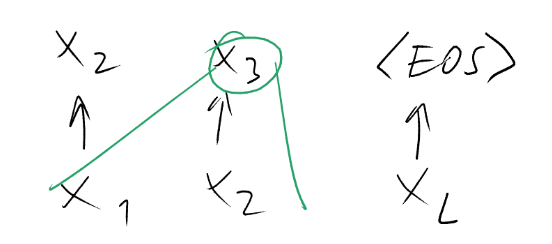
\includegraphics[width=0.5\linewidth]{image.png}
\end{figure}


\textbf{Task}: language modeling, next-token prediction.

$p(x) = p(x_1)\,p(x_2 \mid x_1)\,p(x_3 \mid x_1, x_2)\cdots p(x_L \mid x_1, \ldots, x_{L-1})$

GPT is also suited for generation tasks (e.g. ChatGPT)

\section{BERT (Bidirectional Encoder Representations from Transformers)}
\textbf{Architecture}: Transformer \textit{Encoder} only -- \textbf{bidirectional} (every token sees all tokens)\\
\textbf{Task}: \textit{masked} language modeling (task applies not only for texts and this idea often occurs in self supervised learning).

\subsection*{Masked language modeling (MLM)}

\textbf{Goal:} learn bidirectional context and capture semantic and syntactic structure of language.
Some tokens in the input sequence are randomly masked, and the model is trained to predict them: 

\begin{center}
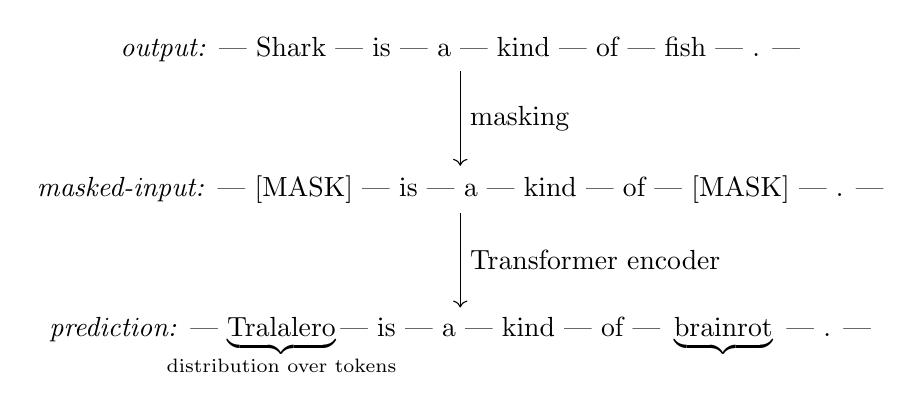
\begin{tikzpicture}[
    node distance=1.2cm,
    arrow/.style={->},
    every node/.style={align=center}
]

\node (a) {\textit{output:} | Shark | is | a | kind | of | fish | . |};

\node (b) [below=of a] {\textit{masked-input:}  | [MASK] | is | a | kind | of | [MASK] | . |};

\node (c) [below=of b] { \textit{prediction:}

| $\underbrace{\text{Tralalero}}_{\mathclap{\text{distribution over tokens}}} \text{| is | a | kind | of | } \underbrace{\text{brainrot}} \text{ | . |}$};
% arrows
\draw[arrow ] (a) -- (b) node[midway, right] {masking};
\draw[arrow, ] (b) -- (c) node[midway, right] {Transformer encoder};

\end{tikzpicture}
\end{center}

The \textbf{original tokens are kept} as \textbf{target values}.\\


The occurring issue is the mismatch between pretraining and inference. During training, some tokens are replaced with [MASK] token, which never appears at test time. This can make the model rely on artificial patterns and lead to suboptimal performance when applied to real text. \\

 \textbf{The solution:} \\
From the input sequence, about \textbf{15\% of tokens} are randomly selected. Each selected token with probability:
\begin{itemize}
    \item[-] 80\% replaced with [MASK] 
    \item[-] 10\%  replaced with a random token
    \item[-] 10\% left unchanged
\end{itemize}

This uncertainty prevents model from overfitting. \\

\textbf{Loss computation}:  \\
! The loss is computed \textbf{only on masked positions} and gradients are computed \textbf{only from the loss at masked tokens}, but they propagate through the entire network.
\\


\textbf{BERT loss}:\\
The overall training objective in BERT is a combination of two tasks:
\[\mathcal{L}_{BERT} = \mathcal{L}_{MLM} + \mathcal{L}_{NSP}\]

MLM:
\begin{itemize}
    \item[+] uses both left and right context;
    \item[+] learns good contextual representations at the token level
    \item[-] bad understanding of \textbf{long-range coherence} or relationships between sentences in a text
\end{itemize}

Since MLM has bad performance on long texts, Bert introduces a second task with additional NSP loss.


\subsection*{Next Sentence Prediction (NSP)}
\textbf{Task:} to predict if sentence S after T or not (binary classification): \\
0 -- $S$ is \textbf{not} the next sentence after $T$ \\
1 --  $S$ \textbf{is} the next sentence after $T$ \\ \\
Let sentence T contain tokens $t_1 \ t_2  \ ...\  t_N$, sentence S contain  $s_1\ s_2\ ...\ s_M$ and some tokens in the input sequence are randomly masked:
\[ \text{\textit{input:  }}{\textbf{[CLS]}}\; t_1\; t_2\; \cancel{t_3}_{\textcolor{orange}{\textbf{[Mask]}}}\; \cdots\; t_N\; \textbf{[SEP]}\; s_1\; s_2\; \cdots\;
\cancel{s_{M-1}}_{\textcolor{orange}{\textbf{[Mask]}}}
\; s_M
\]
BERT is built on a Transformer encoder, and after passing through all self-attention layers, every token gets a contextualized vector.  \\
But since we need \textbf{one vector for the whole input}, not one per token, [CLS] token is always added to the input. \\
A small linear head is placed on top of the final [CLS] vector, and during fine-tuning on other tasks the NSP head is discarded and a new head is placed on top of the same [CLS] vector: 
$$h_{[CLS]} \;\rightarrow\; \text{Linear}(d_{\text{model}} \to 2) \;\rightarrow\; \text{softmax} \;\rightarrow\; \{0,\, 1\}$$

\textbf{Embeddings:} \\
$$E = E_{\text{token}} + E_{\text{position}} + E_{\text{segment}}$$
$$ E_{\text{token}} = E_{[CLS]} + E_{t_1} + E_{t_2} + E_{[MASK]} + \cdots + E_{t_N} + E_{[SEP]}+ E_{s_1} + \cdots + E_{s_{M-1}} + E_{s_M}$$
$$E_{\text{position}} = E_{0} + E_{1} + E_{2} + E_{3}\cdots + E_{N} + E_{N+1}+ E_{N+2} + \cdots +  E_{N+M}+ E_{N+M+1}$$
$$ E_{\text{segment}} = E_{T} + E_{T} + E_{T} + E_{T} \cdots + E_{T} + E_{T}+ E_{S} + \cdots + E_{S} + E_{S}$$

\section{Downstream BERT tasks}

\subsection*{GLUE (General Language Understanding Evaluation)} 
Benchmark -- a collection of 9 NLP tasks (classification):
 
\begin{center}
\begin{tabular}{llp{6cm}}
\toprule 
\textbf{Task} & \textbf{Type} & \textbf{What it tests} \\
\midrule
CoLA  & single sentence & corpus of grammatical acceptability \\
SST-2 & single sentence & sentiment (positive / negative) \\
MRPC  & sentence pair   & paraphrase detection \\
STS-B & sentence pair   & semantic similarity (regression) \\
QQP   & sentence pair   & question paraphrase (Quora) \\
MNLI  & sentence pair   &  \footnotesize{multi-genre Natural Language Inference (NLI)}\\
QNLI  & sentence pair   & QA-based NLI \\
RTE   & sentence pair   & recognising textual entailment \\
WNLI  & sentence pair   & Winograd schema (coreference) \\
\bottomrule
\end{tabular}
\end{center}

Final score -- average across all tasks. \\ (BERT-base achieved 79.6, BERT-large 80.5 and won over GPT at the time).


\subsection*{BERT-like models across modalities}

\textbf{Text}: \\
\href{https://arxiv.org/abs/1907.11692}{RoBERTa} (\textit{arXiv:1907.11692}),
\href{https://arxiv.org/abs/1909.11942}{ALBERT} (\textit{arXiv:1909.11942}) \\
\textbf{Images}: \\
\href{https://arxiv.org/abs/2106.08254}{BEiT} (\textit{arXiv:2106.08254}),
\href{https://arxiv.org/abs/2111.06377}{MAE} (\textit{arXiv:2111.06377}) \\
\textbf{Audio}: \\
\href{https://arxiv.org/abs/2106.07447}{HuBERT} (\textit{arXiv:2106.07447})


\section{SSL for Images}

\textit{ImageNet is too good}\\
Several attempts at self-supervised pretext tasks.

\textbf{Pretext tasks:}
\begin{itemize}
    \item[-] Rotation angle prediction \\ (predict whether the image was rotated by $90^\circ$, $180^\circ$, etc.)
    \item[-] Jigsaw puzzle \\ (shuffle patches of the image; predict the correct permutation)
    \begin{figure}[!h] \centering  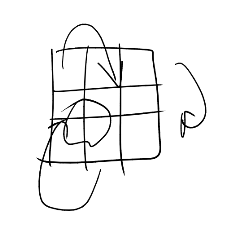
\includegraphics[width=0.15\linewidth]{jigsaw.png} \end{figure}
    \item[-] Image colorization (grayscale $\rightarrow$ color)
\end{itemize}

Moderate success, ImageNet is still king. Let's proceed to something that really works.

\subsection*{Triplet Loss}
The goal is to train an embedding function $f$ such that similar inputs are close
and dissimilar inputs are far apart in embedding space (Used in e.g.\ \textbf{FaceNet}).

\textbf{Three elements of a triplet:}
\begin{itemize}
    \item[-] $A$ -- anchor
    \item[-] $P$ -- positive (same class as $A$)
    \item[-] $N$ -- negative (different class)
\end{itemize}

$$ \mathcal{L} = \max\!\left(\|f(A) - f(P)\|_2^2 - \|f(A) - f(N)\|_2^2 + m,\; 0\right)$$

We want the negative to be farther from the anchor than the positive, with a margin $m$:\[ m < \|f(A) - f(N)\|_2^2 - \|f(A) - f(P)\|_2^2 \]
If this is satisfied, loss is zero, no gradient.\\ 
Margin $m > 0$ prevents the model from collapsing all embeddings to a single point (similar to gradient clipping).


\section{Contrastive Learning}

\textbf{SimCLR} (A Simple Framework for Contrastive Learning of Representations, \href{https://arxiv.org/abs/2002.05709}{\textit{arXiv:2002.05709}})

 Given a batch $\{x_i\}_{i=1}^{N}$ from sample $\{x_i\}_{i=1}^{L}$, apply two \textbf{random} augmentations $A(\cdot)$ and  $A'(\cdot)$ to each sample:
\[
x_i \;\xrightarrow{A(\cdot)}\; \tilde{x}_i, \qquad x_i \;\xrightarrow{A(\cdot)}\; \tilde{x}_{i+N}
\]
This gives a \textbf{double batch} $\{\tilde{x}_i\}_{i=1}^{2N}$ of augmented views.

Then:
\[
\tilde{x}_i \;\rightarrow\; f(\cdot) \;\rightarrow\; t_i \;\rightarrow\; g(\cdot) \;\rightarrow\; z_i
\]
where $f$ is the backbone encoder, $t_i$ are the embedings, and $g$ is a small projection head. The head $g$ is \textbf{dropped before fine-tuning}; representations $t_i$ are used downstream. We want to maximize agreement between $z_i$ and $z_{i+N}$.

\begin{figure}[!h]
    \centering
    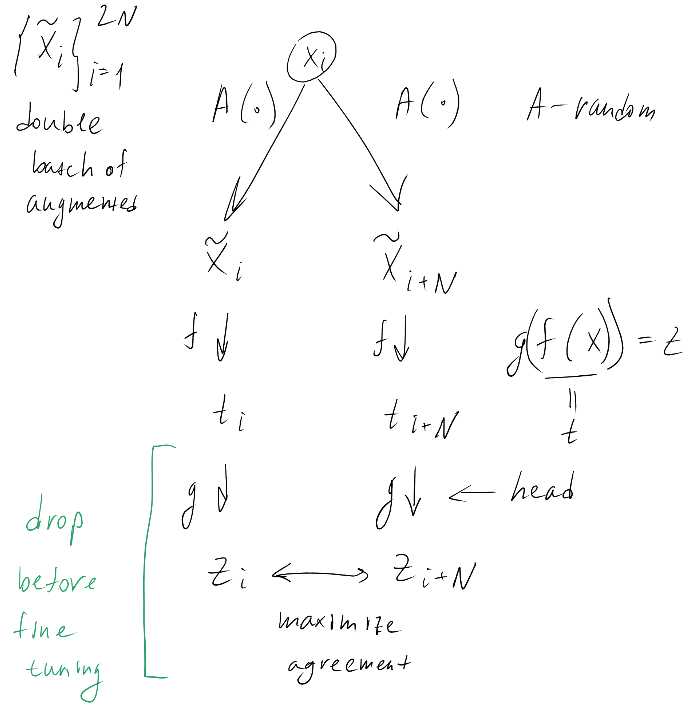
\includegraphics[width=1\linewidth]{im.png}
\end{figure}

For each pair $(z_i, z_{i+N})$ (two views of the same image):
\begin{itemize}
    \item[-] $z_i, z_{i+N} \rightarrow $\textit{close} (positive pair)
    \item[-] $z_i, z_j$ for $j \neq i, j \neq i{+}N \rightarrow$ \textit{far} (negative pairs)
\end{itemize}

\textbf{Loss}:
$$
    l(z_i, z_{i+N}) = -\log \frac{\exp\!\left(\operatorname{sim}(z_i, z_{i+N})\right)}
    {\displaystyle\sum_{k=1}^{2N} \mathbb{1} [k \neq i,\, i{+}N]\, \exp\!\left(\operatorname{sim}(z_i, z_k)\right)}
    \longrightarrow \min_{f,\, g}
$$
where $\operatorname{sim}(u, v) = \dfrac{u^\top v}{\|u\|\|v\|}$ is cosine similarity.

The final loss is symmetrised over both views:
$$
    L(z_i, z_{i+N}) = \frac{1}{2}\Bigl(\ell(z_i, z_{i+N}) + \ell(z_{i+N}, z_i)\Bigr)
$$

We need to pick strong augmentations so the model can train: \\
$(A(x), x)$ -- images are still similar \\
$(A(x), A'(x))$ -- images are more distant!

\textbf{Augmentations $A(\cdot)$:}
\begin{itemize}
    \item Random crop
    \item Color jitter
    \item Convert to grayscale
    \item Gaussian blur
\end{itemize}

\end{document}
